\textbf{7.6}
Interpolating the data points
\begin{table}[H]
  \centering
\begin{tabular}{c|ccccccccc}
  $t$ & 0 & 1 & 4 & 9 & 16 & 25 & 36 & 49 & 64
  \\
  $y$ & 0 & 1 & 2 & 3 & 4 & 5 & 6 & 7 & 8
\end{tabular}
\end{table}
should give an approximation to the square root function.
\begin{itemize}
\item[(a)]
  Compute the polynomial of degree eight that interpolates these nine data points.
  Plot the resulting polynomial as well as the corresponding values given by the
  built-in \verb|sqrt| function over the domain $[0, 64]$.
\item[(b)]
  Use a cubic spline routine to interpolate the same data and
  again plot the resulting curve along with the built-in \verb|sqrt| function.
\item[(c)]
  Which of the two interpolants is more accurate over most of the domain?
\item[(d)]
  Which of the two interpolants is more accurate between $0$ and $1$?
\end{itemize}
\begin{sol}
  \begin{multicols}{2}
    \begin{itemize}
      \item[(a)]
        \setlength{\columnseprule}{0.2pt}
          The code and the plot are shown as follows.
          \lstinputlisting[firstnumber=1]{matlab/polyinterp.m}

              \begin{figure}[H]
      \centering
      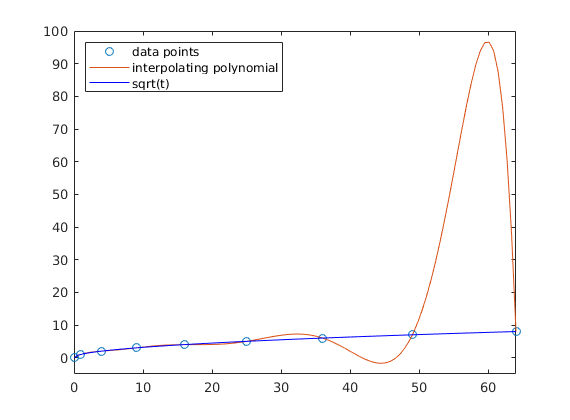
\includegraphics[scale=0.48]{png/polyinterp.png}
    \end{figure}

  \item[(b)]
    The code and the plot are shown as follows.
    \lstinputlisting[firstnumber=1]{matlab/cubicSpline.m}
    \begin{figure}[H]
      \centering
      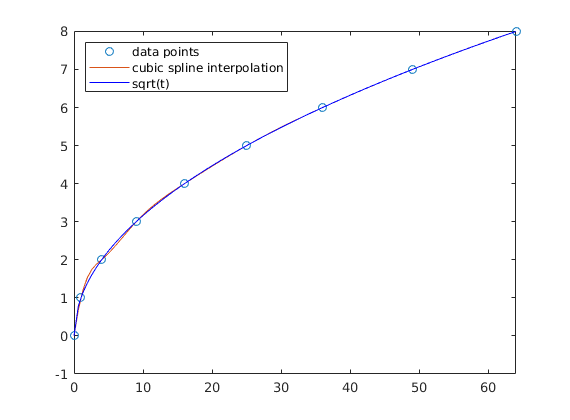
\includegraphics[scale=0.48]{png/cubicSpline.png}
    \end{figure}

  \item[(c)]
    From the above two figures,
    we see that the cubic spline interpolant is more accurate over most of the domain.

  \item[(d)]
    The polynomial interpolant is slightly more accurate between $0$ and $1$,
    as illustrated by the following figure.
    \begin{figure}[H]
      \centering
      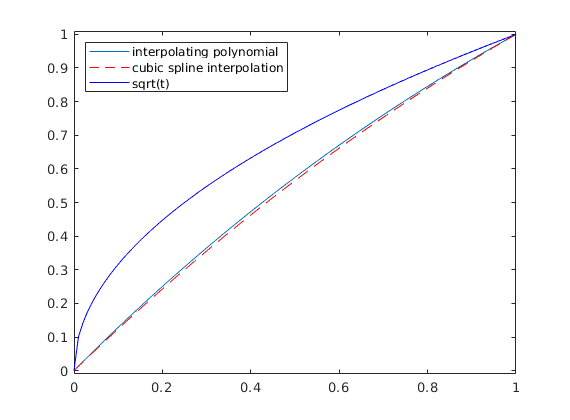
\includegraphics[scale=0.48]{png/interp2.png}
    \end{figure}
  \end{itemize}    
\end{multicols}
\end{sol}
%%% Local Variables:
%%% mode: latex
%%% TeX-master: "../ComputerAssignment"
%%% End:
